\documentclass[9pt]{beamer}

\usepackage[utf8]{inputenc}
\usepackage{eurosym}
\RequirePackage[francais]{babel}
%\usepackage{url}
%\usepackage{etex}
%\usepackage{enumitem}
%\usepackage{multicol}
\usepackage{xcolor}
%\usepackage{bbm}
%\usepackage{amsmath,amsthm,amssymb}
%\usepackage[official]{eurosym}
%\usepackage{pifont}
%\usepackage{exercise}
%\usepackage{graphics}
%\usepackage{array,multirow,makecell}
\usepackage{verbatim}
%\usepackage[dvipsnames]{pstricks}
\usepackage{pstricks-add,pst-plot,pst-text,pst-tree,pst-eps,pst-fill,pst-node,pst-math,pst-blur,pst-func}
%\usepackage{pgf,tikz}
%\usepackage{tipfr}
%\usepackage{thmbox}
%\usepackage{calc}
%\usepackage{ifthen}
%\usepackage{pdfpages}
%\usepackage{colortbl}
%\usepackage{sagetex}
%\usetikzlibrary{arrows,patterns}
%\input tabvar
%\usepackage{tkz-tab}
%\usepackage{listings}
%\usepackage[np]{numprint}
%\usepackage{fancybox,fancyhdr}
%\usepackage{thmtools}
%\usepackage{bclogo}
%\usepackage{lastpage}

\usepackage{tabularx}
\usepackage{array,multirow,makecell}
\usetheme{Madrid}
%\usetheme{Bergen}
\usecolortheme{beaver}
 
%Information to be included in the title page:
\title{Python}
\subtitle{Tuples - Tableaux - Listes}
\author{Yannick CHISTEL}
\institute{Lycée Dumont d'Urville - CAEN}
\date{Décembre 2019}
 
%----------------------------------------------------------------------------------------------- 
% 							Commandes Tableaux
%-----------------------------------------------------------------------------------------------
\setcellgapes{1pt}
\makegapedcells
\newcolumntype{R}[1]{>{\raggedleft\arraybackslash }b{#1}}
\newcolumntype{L}[1]{>{\raggedright\arraybackslash }b{#1}}
\newcolumntype{C}[1]{>{\centering\arraybackslash }b{#1}}

\definecolor{vert}{rgb}{0,0,1}


\newcounter{num}
\setcounter{num}{0}
 
\begin{document}
 
\frame{\titlepage}

\begin{frame}
\frametitle{Tableaux}


\begin{block}{Données multiples}
Une variable contient une valeur, modifiable à tout moment dans le programme.

Il est parfois nécessaire de créer de très nombreuses variables du même type. Par exemple, les jours de la semaine, les mois de l'année, les dates...

\begin{itemize}
\item j1="lundi", j2="mardi", j3="mercredi", ...
\item m1="janvier", m2="février", m3="mars", ...
\item d1=1, d2=2, ..., d31=31
\end{itemize}

Les tableaux sont une structure en informatique qui permettent de stocker toutes les valeurs dans une même variable.

\begin{itemize}
\item jours="lundi", "mardi", "mercredi", ..., "dimanche"
\item mois="janvier", "février", "mars", ..., "décembre"
\item dates=1, 2, 3, ..., 31
\end{itemize}


En \textbf{python}, il en existe 2 types de tableaux : les \textbf{tuples} et les \textbf{listes}.
\end{block}

%\begin{exampleblock}{Exemple}
%\begin{itemize}
%\item Le réseau électrique : Centrales, câbles, logements
%\item Le réseau ferroviaire : Gares et voies ferrées
%\item Un réseau hydraulique : Pompe, canalisations, robinetterie
%\end{itemize}
%\end{exampleblock}
%
%\begin{block}{Réseau informatique}
%Dans un réseau informatique :
%\begin{itemize}
%\item Les \textbf{noeuds} sont les ordinateurs, serveurs, routeurs, commutateurs, tablettes téléphones,...
%\item Les \textbf{liens} sont les câbles de cuivre, fibre optique et les ondes (wifi, bluetooth, 4G, 5G,...)
%\end{itemize}
%\end{block}

\end{frame}


\begin{frame}
\frametitle{Tableaux python}

\begin{block}{Tuple et Liste}
Un \textbf{tuple} ou une \textbf{liste} regroupe plusieurs valeurs dans une \textbf{même variable}.

Un \textbf{tuple} se note entre \textbf{parenthèses} contenant les valeurs séparées par des virgules.

Une \textbf{liste} se note entre \textbf{crochets} contenant les valeurs séparées par des virgules.

%Chaque valeur d'un tuple ou d'une liste est indicée. On accède aux valeurs en se référant à l'indice.
\end{block}

\begin{exampleblock}{Exemple}
Les différentes variables utilisées pour les jours de la semaine peuvent être rassemblées dans une même variable en \textbf{tuple} ou en \textbf{liste}.
\begin{enumerate}
\item Pour un \textbf{tuple} (avec des parenthèses) :
\textbf{jours}=("lundi","mardi","mercredi","jeudi","vendredi","samedi","dimanche")
\item Pour une \textbf{liste} (avec des crochets) :
\textbf{jours}=["lundi","mardi","mercredi","jeudi","vendredi","samedi","dimanche"]
\end{enumerate}
\end{exampleblock}


\begin{alertblock}{Remarque importante}
\begin{enumerate}
\item Un \textbf{tuple} n'est pas modifiable. On ne peut pas modifier les valeurs.

Un tuple n'est pas \textbf{mutable}.

\item Une \textbf{liste} est modifiable. On peut modifier les valeurs.

Une liste est \textbf{mutable}.
\end{enumerate}

\end{alertblock}

\end{frame}


\begin{frame}
\frametitle{Tableaux python}

\begin{block}{Création d'un tableau}
Pour créer un \textbf{tuple} ou une \textbf{liste}, il suffit d'écrire les valeurs séparées par des virgules entre \textbf{parenthèses} pour un \textbf{tuple} et entre \textbf{crochets} pour une \textbf{liste}.
\end{block}

\begin{exampleblock}{Exemple}
Les mois de l'année (de type "string") :

Sous forme de tuple : \textbf{mois}=("janvier", "février", ... , "novembre", "décembre")

Sous forme de liste : \textbf{mois}=["janvier", "février", ... , "novembre", "décembre"]

\end{exampleblock}

\begin{block}{Longueur d'un tableau}
Pour accéder à une valeur d'un tuple ou d'une liste, on utilise son indice (index en anglais). Il est donc important de connaître la \textbf{longueur} d'un tableau, c'est à dire le nombre de ses éléments.\smallskip

En \textbf{python}, la longueur d'un tuple ou d'une liste est donnée avec la fonction \textbf{len}.
\end{block}

\begin{exampleblock}{Exemple}
\textbf{len}(mois) renvoie $12$, donc le tableau contient 12 éléments \textbf{indicés} de 0 à 11.

\textbf{mois}[\textbf{0}] vaut "janvier", \textbf{mois}[\textbf{1}] vaut "février", ... , \textbf{mois}[\textbf{11}] vaut "décembre"
\end{exampleblock}

\end{frame}




\begin{frame}
\frametitle{Parcourir un tableau}

\begin{block}{Méthode}
On peut parcourir un tableau et donc récupérer ses valeurs en itérant sur les indices avec une boucle. Soit tab une variable de type tableau :
\begin{enumerate}
\item Avec une boucle \textbf{for} :

\textbf{for} i \textbf{in range}(\textbf{len}(tab)):

\hspace{0.5cm} ... tab[i] ...

\item Avec une boucle \textbf{while} :

\textbf{while} k $<$ \textbf{len}(tab):

\hspace{0.5cm} ... tab[k] ...

\hspace{0.5cm} k = k+1
\end{enumerate}
\end{block}

\begin{exampleblock}{Exemple}
Afficher les mois de l'année avec une boucle for : \smallskip

\textbf{for} i \textbf{in range}(\textbf{len}(mois)):

\hspace{0.5cm} \textbf{print}(mois[i],end="-")\smallskip
    
qui affichera : 

janvier-février-mars-avril-mai-juin-juillet-septembre-octobre-novembre-décembre-
\end{exampleblock}

\end{frame}


\begin{frame}
\frametitle{Valeurs d'une liste}

\begin{block}{Méthode 1}
On peut modifier les valeurs d'une liste en affectant directement les nouvelles valeurs repérées par leurs indices.
\end{block}

\begin{exampleblock}{Exemple}
Soit la liste des jours de la semaine dans la variable jours:

\hspace{0.5cm}\textbf{jours} = ("lundi", "mardi", "mercredi", "jeudi", "vendredi", "samedi", "dimanche")

Si on souhaite remplacer les valeurs de la liste jours par des valeurs en anglais :\\
jours[0]="monday", jours[1]="tuesday", etc
\end{exampleblock}

\begin{block}{Méthode 2}
Si on souhaite construire un tableau de très grande taille, python permet une construction rapide avec des valeurs initiales:

\hspace{0.5cm} variable tableau = [valeur initiale] * dimension du tableau
\end{block}

\begin{exampleblock}{Exemple}
Construire une liste de 100 nombres : \hspace{0.25cm}\textbf{nombres} = [0] * 100

On a un tableau rempli de 100 zéros : [0,0,0,...0,0]
\end{exampleblock}
\end{frame}

\begin{frame}
\frametitle{Tableaux et variables}

\begin{block}{Variables}
\begin{minipage}{0.7\textwidth}
\begin{enumerate}
\item Soit $x$ et $y$ deux variables.\\
On affecte les variables : $x=2$ et $y=x$. On a 2 espaces mémoires distincts qui ont la même valeur.\\
Si maintenant on a $x=5$ alors $y$ vaut toujours $2$.
\item Soit la variable tableau $t$ contenant les valeurs $1$, $2$, $3$.\\
Si on déclare une seconde variable tableau $u$ en lui affectant la valeur de la variable $t$: $u=t$.\\
Dans ce cas, les variables $t$ et $u$ désignent le même tableau !\\
Si on modifie la valeur $u[1]=0$ alors $t[1]=0$.
\end{enumerate}
\end{minipage}\hfill
\begin{minipage}{0.28\textwidth}
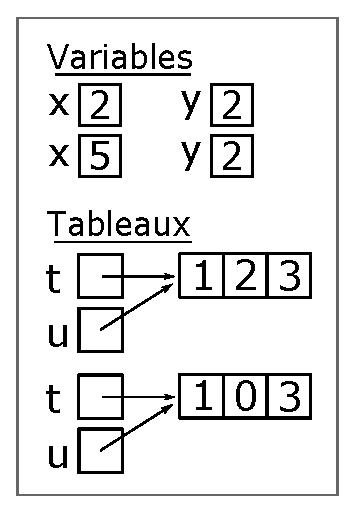
\includegraphics[scale=0.5]{img/tableaux.eps}
\end{minipage}
\end{block}


\begin{alertblock}{Remarque}
Cette affectation par égalité de tableaux lie les deux tableaux. Mais à tout moment on peut délier les tableaux en affectant un nouveau tableau à l'une des variables.

Par exemple : $u=[7,8,9]$ du coup on redéfinit un nouveau tableau ! $u$ et $t$ ne sont plus liés.
\end{alertblock}

\end{frame}


\begin{frame}
\frametitle{Tableaux et fonctions}

\begin{block}{Présentation}
\begin{enumerate}
\item Une fonction accepte un tableau comme paramètre. Dans ce cas, la fonction peut modifier le tableau.
\item Une fonction peut retourner un tableau de valeurs.
\end{enumerate}

\end{block}

\begin{exampleblock}{Exemple}
\begin{minipage}{0.45\textwidth}
\textbf{def} carres(n):

\hspace{0.5cm}t=[0]*n

\hspace{0.5cm}\textbf{for} i in \textbf{range}(n):

\hspace{1cm}t[i]=(i+1)**2

\hspace{0.5cm}\textbf{return} t
\end{minipage}\hfill
\begin{minipage}{0.45\textwidth}
\textbf{def} quadro(t):

\hspace{0.5cm}\textbf{for} i in range(len(t)):

\hspace{1cm}t[i]=t[i]**2

\hspace{0.5cm}\textbf{return} t\\
\end{minipage}
\medskip

\begin{enumerate}
\item Si une variable \textbf{c} = \textbf{carres(5)}, celle-ci a pour valeur le tableau [1,4,9,16,25].
\item Si on appelle la fonction \textbf{quadro(c)}, la variable c a pour valeur le tableau [1, 16, 81, 256, 625].
\end{enumerate}
\end{exampleblock}

\begin{alertblock}{Attention}
Dans les fonctions, les tableaux sont directement modifiés et cela nécessite de la réflexion et des tests.
\end{alertblock}

\end{frame}

%****************************************************************************
%
% Partie 2 : tableaux avancés
%
%****************************************************************************

%Information to be included in the title page:
\title{Python}
\subtitle{Seconde partie :\\\medskip Utilisation avancée des tableaux}
\author{}
\institute{}
\date{}

\frame{\titlepage}

\begin{frame}
\frametitle{Parcourir un tableau}

\begin{block}{Tableaux et indices négatifs}
%On accède aux éléments d'un tableau avec leurs indices.

On peut accéder aux derniers éléments d'un tableau avec des indices négatifs :
\begin{itemize}
\item liste[0] : première valeur du tableau
\item liste[-1] : dernière valeur du tableau
\item liste[-2] : avant-dernière valeur du tableau
\end{itemize}

%\begin{tabular}{|L{2.2cm}*{5}{|C{1.2cm}}|}\hline
%Tableau & Valeur 1& Valeur 2 & & Valeur n\\\hline
%Indices positifs & 0 & 1 & & n-1\\\hline
%Indices négatifs & -(n-1) & &-2&-1\\\hline
%\end{tabular}
\end{block}

\begin{block}{Itérer sur les éléments}
%On accède aux éléments d'un tableau avec leurs indices. 
On peut accéder à un élément d'une liste avec une boucle for et la syntaxe suivante :

\textbf{for} e \textbf{in} liste:

\hspace{0.5cm}instruction avec e

\end{block}

\begin{exampleblock}{Exemple}
Soit t=[1,2,3,4,5,6]
\begin{enumerate}
\item \textbf{print(t[-1])} affiche la valeur 6
\item \textbf{print(t[-2])} affiche la valeur 5
\item \textbf{for} k \textbf{in} t:

\hspace{0.5cm}\textbf{print}(k, end=' ') affiche 1 2 3 4 5 6
\end{enumerate}

\end{exampleblock}

\end{frame}


\begin{frame}
\frametitle{Créer un tableau par \textbf{compréhension}}

\begin{block}{Création d'un tableau}
La construction d'un tableau par compréhension introduit la boucle for à l'intérieur des crochets du tableau à construire. La syntaxe est de la forme:

\hspace{0.5cm} [valeur \textbf{for} i \textbf{in range}(dimension du tableau)]
\end{block}

\begin{exampleblock}{Exemple}
\begin{enumerate}
\item Construire par compréhension une liste ordonnée de nombres:
\begin{enumerate}
\item[a)] [i \textbf{for} i in range(5)] construit le tableau [0, 1, 2, 3, 4]
\item[b)] [i**2 \textbf{for} i in range(5)] construit le tableau [0, 1, 4, 9, 16]
\item[c)] [2*i+1 \textbf{for} i in range(5)] construit le tableau [1, 3, 5, 7, 9]
\end{enumerate}
\item Construire un tableau à partir des valeurs d'un autre tableau :\\
t=[2,3,5,7,11,13]\\
p=[x**2 \textbf{for} x in t]\\
Le tableau p a pour valeur [4, 9, 25, 49, 121, 169] 
\item Construire un tableau dont les valeurs sont des chaines de caractères:\\
direction=['nord','sud','est','ouest']\\
DIRECTION=[e.upper() for e in direction]\\
Le tableau DIRECTION a pour valeur ['NORD', 'SUD', 'EST', 'OUEST']
\end{enumerate}
\end{exampleblock}

\end{frame}




\begin{frame}
\frametitle{Copier un tableau : \textbf{list}}

\begin{block}{Méthode}
On a vu que la copie d'un tableau ne se fait pas par affectation puisque les variables vont au final désigner le même tableau.

Pour déclarer une nouvelle variable en lui affectant les valeurs d'un tableau existant, on utilise la fonction \textbf{list} avec la syntaxe :

tableau2 = \textbf{list}(tableau1)

\end{block}

\begin{exampleblock}{Exemple}
t=[10,20,30,40,50] \\
u=\textbf{list}(t)\\
\textbf{print}(u) affiche [10,20,30,40,50]  \hspace{1cm}  \textit{le tableau est copié dans la variable u.}\\
\textbf{for} i \textbf{in range}(5):\\
\hspace{0.5cm}u[i]=u[i]/10  \hspace{1cm}  \textit{ici, chaque valeur de u est divisée par 10}\\
\textbf{print(t)} afffiche [10,20,30,40,50]  \hspace{1cm} \textit{ le tableau t n'a pas changé}\\
\textbf{print(u)} afffiche [1,2,3,4,5]  \hspace{1cm} \textit{ le tableau u a ses valeurs divisées par 10}
\end{exampleblock}

\end{frame}


\begin{frame}
\frametitle{Modifier les tableaux}

\begin{block}{Ajouter des valeurs}
Un tableau est de dimension fixée. Mais, en python, il est possible d'agrandir un tableau en ajoutant des valeurs. Deux méthodes sont possibles :
\begin{enumerate}
\item Par concaténation de deux tableaux existants avec l'opérateur + ;
\item En utilisant la fonction \textbf{append} qui permet d'ajouter une valeur en fin de tableau.
\end{enumerate}
\end{block}

\begin{exampleblock}{Exemple}
\begin{enumerate}
\item Par concaténation de tableaux :\\
t=[0,1,2]\\
u=[3,4,5]\\
s=t+u \hspace{1cm} \textit{le tableau u a pour valeur [0,1,2,3,4,5]}
\item Avec la fonction \textbf{append} :
t=[0,1,2]\\
t.append(3) \hspace{1cm} \textit{le tableau t a pour valeur [0,1,2,3]}\\
t.append(4) \hspace{1cm} \textit{le tableau t a pour valeur [0,1,2,3,4]}
\item Avec la fonction \textbf{append} et une boucle \textbf{for}:
t=[0,1,2]\\
u=[3,4,5]\\
\textbf{for} e in u:\\
\hspace{0.5cm}t.append(e) \hspace{1cm} \textit{le tableau t a pour valeur [0, 1, 2, 3, 4, 5]}
\end{enumerate}
\end{exampleblock}

\end{frame}

\begin{frame}
\frametitle{Des fonctions sur les tableaux}

\begin{block}{Présentation}
Il existe des fonctions que l'on peut appliquer sur un tableau, pour ajouter des éléments (append) et pour connaître le nombre d'éléments (len). En voici d'autres fonctions (liste non exhaustive):
\begin{itemize}
\item La fonction copy qui recopie les valeurs d'un tableau dans un autre ;\\
\item La fonction pop qui supprime la dernière valeur d'un tableau ;
\item La fonction insert qui insère une valeur pour un indice donné du tableau ;
\item La fonction remove qui suprrime une valeur pour un indice donné du tableau ;
\item La fonction sort trie le tableau dans l'ordre croissant.
\end{itemize}
\end{block}

\begin{exampleblock}{Exemple}
Soit un tableau : t=[0,1,2,3]
\begin{enumerate}
\item u=t.copy() \hspace{1cm} \textit{le tableau u est créé et a les mêmes valeurs que t}
\item u.pop() \hspace{1cm} \textit{la dernière valeur du tableau u est supprimée ; u vaut [0,1,2]}
\item u.insert(1,4) \hspace{1cm} \textit{la valeur 4 est insérée à l'indice 1 ; u vaut [0,4,1,2]}
\item u.remove(1) \hspace{1cm} \textit{si elle existe, la valeur indiquée est supprimée ; u vaut [0,4,2]}
\item u.sort() \hspace{1cm} \textit{le tableau u est trié ; u vaut [0,2,4]}
\end{enumerate}
\end{exampleblock}

\end{frame}


\begin{frame}
\frametitle{Tableau de tableaux}

\begin{block}{Présentation}
Un tableau peut contenir tout type de valeurs: des entiers (int), des chaines de caratères (string), des nombres réels (float) et aussi des tableaux !\medskip

Pour accéder à une valeur de ce tableau, on utilise un premier indice pour sélectionner le tableau où se trouve la valeur puis un second indice pour obtenir la valeur dans le tableau sélectionné. Les indices sont notés entre crochets.
\end{block}

\begin{exampleblock}{Exemple}
\begin{enumerate}
\item t=[[4,5],[6,7],[8,9]]\\
Le tableau t contient 3 tableaux de dimension 2 ; t est un tableau de dimension $3 \times 2$ ;\\
le tableau [4,5] est d'indice 0, le tableau [6,7] d'indice 1 et le tableau [8,9] d'indice 2 ;\\
les valeurs ont pour indice 0 et 1 pour chacun des trois tableaux ;\\

\textbf{print}(t[1][0]) \hspace{1cm} \textit{tableau d'indice 1, valeur d'indice 0 ; affiche la valeur 6}
\item On initialise un tableau de tableaux par compréhension :\\
t=[ [0]*3 for i in range(3) ] \hspace{1cm} le tableau t vaut [ [0,0,0], [0,0,0], [0,0,0] ]
\end{enumerate}

\end{exampleblock}

\end{frame}

\end{document}

